\section{Tip reconstruction - image deconvolution}

\paragraph{Erosion algorithm: }

The erosion algorithm, as introduced by Villarubbia \cite{scanning_microscope,Villarrubia}, is aimed at reconstructing the tip shape based on both the actual and the ideal topography data. This algorithm, known as the naive erosion method, was initially devised to determine the covering envelope of a sphere as it moves across a surface. The envelope essentially represents the path traced by the center of the sphere as it rolls over the sampled points on the surface.

Notice that, although the structuring element in this specific implementation is a sphere, it is important to highlight, in a broader context, that this algorithm can be extended to many other shapes such as bipyramids, nanosheets, and more. When considering these alternative shapes, it becomes challenging to visualize how they would interact with the surface in a rolling motion. Therefore, it is more accurate to describe the interaction of the structuring element with the surface as a planar displacement rather than a rolling action.

\paragraph{Mathematical solution: }

The algorithm takes two key inputs: the surface to undergo erosion (denoted as S) and the structuring element (denoted as B). Then it applies the erosion equation (reflected in Equation \ref{eq:erosion}) to each pair of coordinates (u, v) within the topography data.

\begin{equation}
    \label{eq:erosion}
    T(x, y) = S \ominus B = \min_{u, v}\left(S(x + u, y + v) - B(u, v)\right)
\end{equation}

Basically, the naive erosion algorithm aligns with the principles of morphological dilation and erosion (as shown in Fig. \ref{fig:filter}), which are essentially defined as the Minkowski addition and subtraction operations \cite{erosion_Minkowskische} between the input set and the structuring element, respectively. This mathematical framework underpins the process of shape transformation and reconstruction within the context of the erosion algorithm.

\begin{figure}[ht]
    \centering
    \begin{subfigure}[b]{0.45\textwidth}
        \includegraphics[width=.98\textwidth]{./immagini/erosion2.png}
        \caption{}
        \label{fig:filter_a}
    \end{subfigure}
    \hfill
    \begin{subfigure}[b]{0.45\textwidth}
        \includegraphics[width=.98\textwidth]{./immagini/erosion3.png}
        \caption{}
        \label{fig:filter_b}
    \end{subfigure}
    \caption{Morphological filters (The structuring element is the apex tip): b) Dilation process on a sample profile c) Erosion process on a sample profile}
    \label{fig:filter}
\end{figure}

\newpage

In the following Fig. \ref{fig:confronto_pre_post} the original topography (a) and the deconvoluted result (b) of the naive erosion algorithm are shown.

\begin{figure}[ht]
    \centering
    \begin{subfigure}[b]{0.40\textwidth}
        % 2
        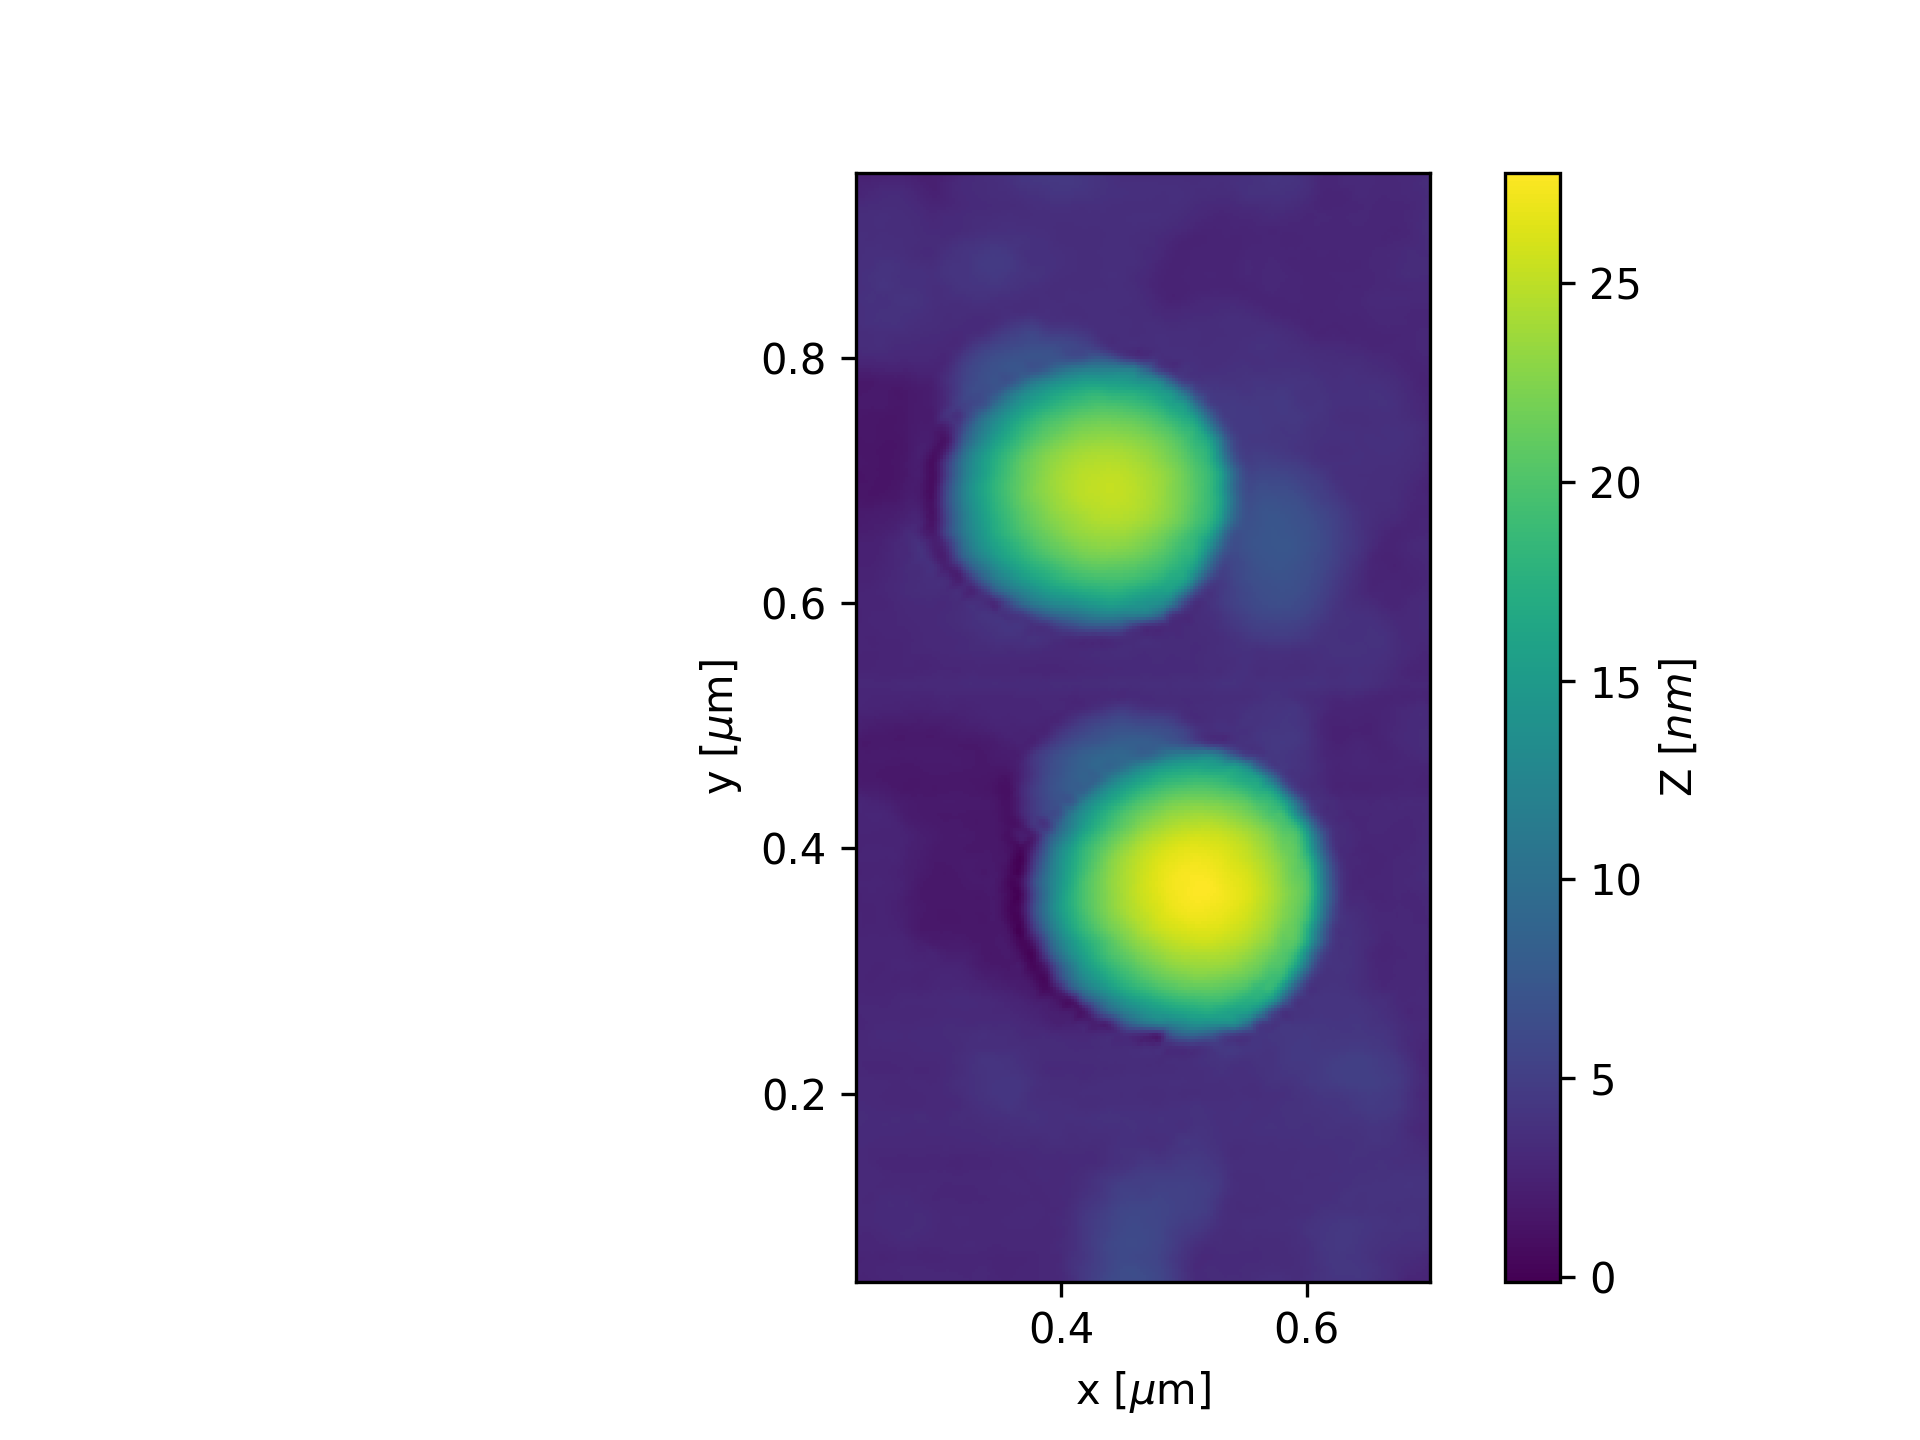
\includegraphics[width=.95\textwidth, trim={170, 0, 40, 0}, clip]{./immagini/2.png}
        \caption{}
        \label{fig:prima}
    \end{subfigure}
    \hfill
    \begin{subfigure}[b]{0.40\textwidth}
        % 4
        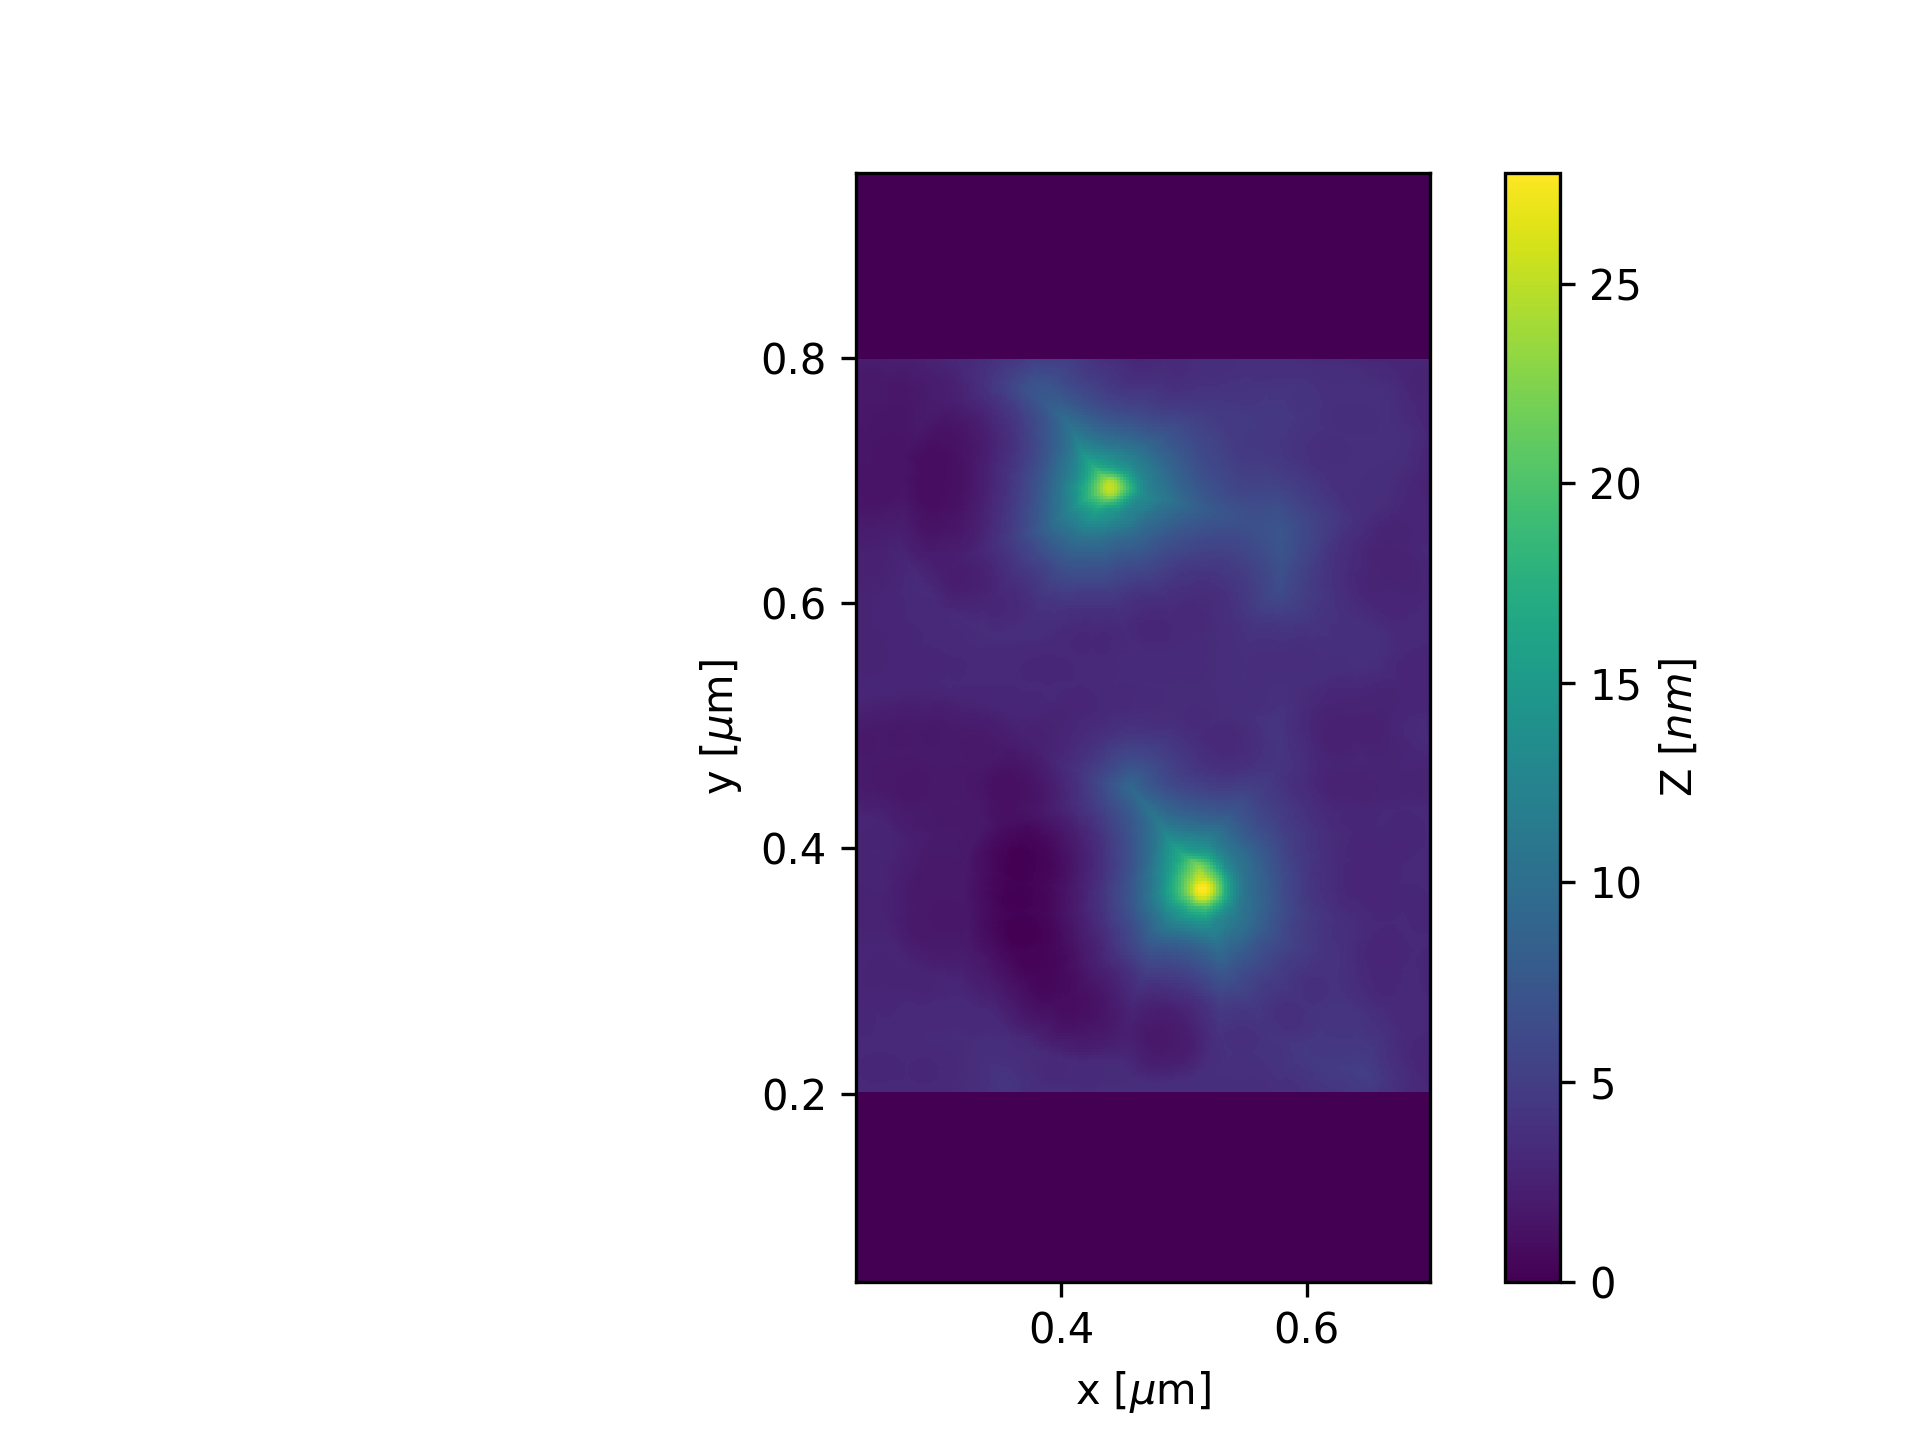
\includegraphics[width=.95\textwidth, trim={170, 0, 40, 0}, clip]{./immagini/4.png}
        \caption{}
        \label{fig:dopo}
    \end{subfigure}
    \caption{Results a) Original Data b) Deconvoluted image}
    \label{fig:confronto_pre_post}
\end{figure}

In Fig. \ref{fig:tiptredi}, the reconstructed tip, as obtained from just the Minkowski subtraction, is shown. 

\begin{figure}[ht]
    \centering
    % punta_finale
    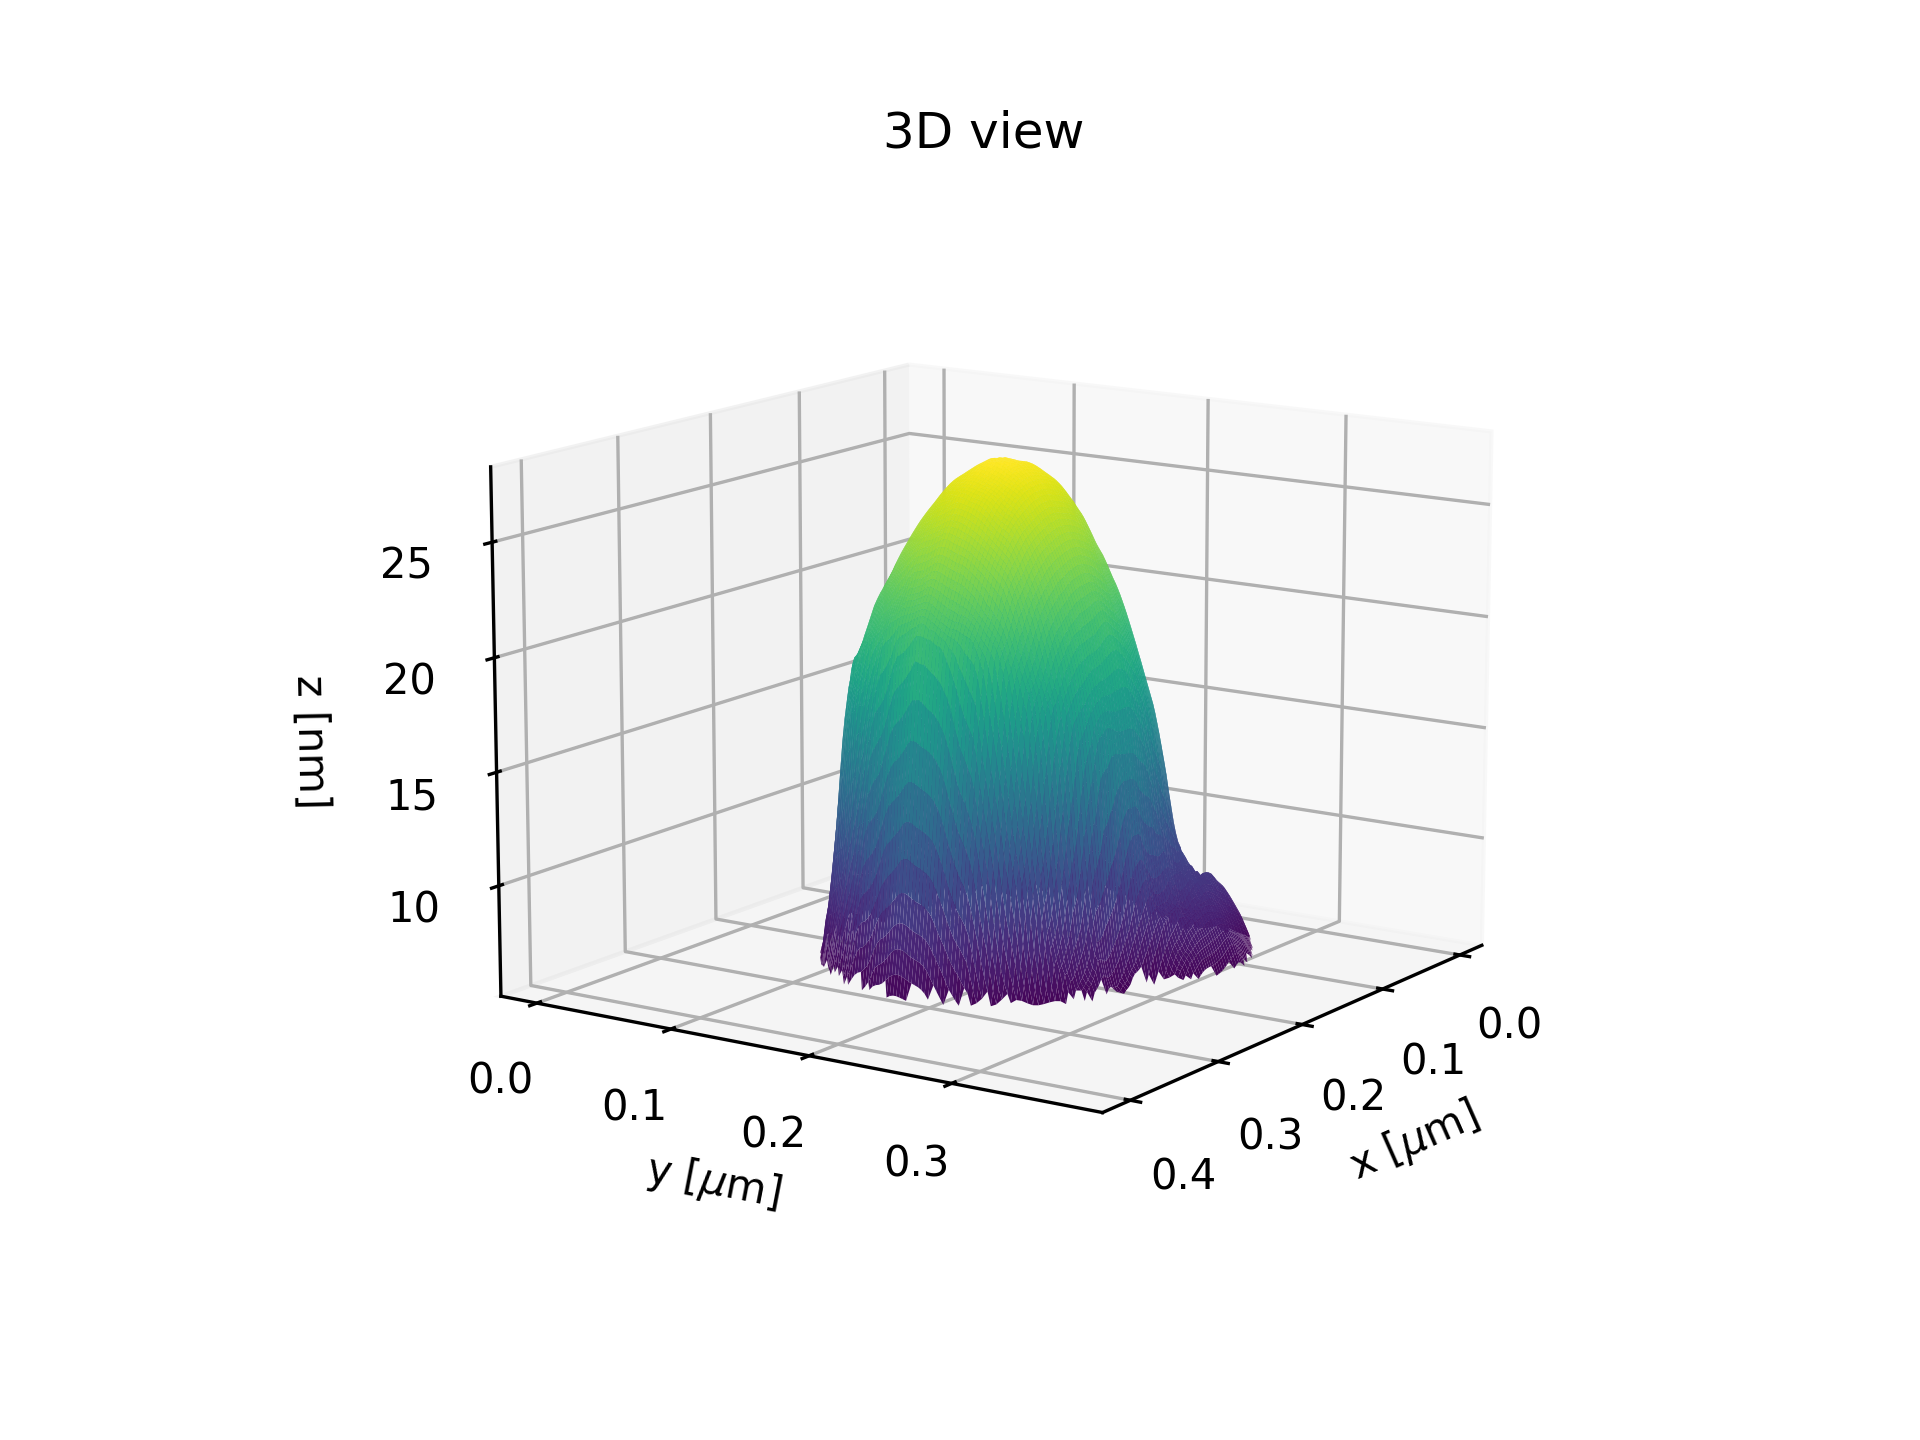
\includegraphics[width=.7\textwidth]{./immagini/punta_finale.png}
    \caption{Reconstructed 3D tip}
    \label{fig:tiptredi}
\end{figure}